\section{Usability}
In their current state, unikernels are not as usable as easy as docker containers. Docker, or container technology in general, has a working abstraction between code and infrastructure. Unikernels currently lack that abstraction. If a unikernel supports a certain language, then the application code should also be in that language. MirageOS is written in OCaml and all the libraries are also written in OCaml. That's why it only supports applications in OCaml. That makes it really hard for someone to develop applications if they are not familiar with the language. This makes sense that the application code blends in perfectly with the operating system it's being built into, nevertheless it restricts developers to develop programs in broad sense. OCaml was not on the list for the most loved 25 programming languages survey of Stack Overflow for 2019 \cite{2019-survey}.

The networking in unikernels is also different than what we use in docker containers. Docker containers are system processes and connecting processes through ports is well established in computer engineering. Unikernels have their own networking stack for each hypervisor and they are not unified. Bonk et al. \cite{Bonk} explains how certain networking stacks are implemented in MirageOS and how they differ from each other. For every deployment, developer has to come up with a custom solution for networking.

On the other hand, there are projects where MirageOS was used for superior functionality. An example project is called Jitsu\cite{jitsu}, Just in time summoning of unikernels. In that project, for every DNS request, they are starting a unikernel to respond to that request by returning the newly acquired IP of the unikernel with the response header. The working principle can be seen in \ref{fig:jitsu}.

\begin{figure}[h!]
\centering
\begin {sequencediagram}
  \newinst {client}{Client}
  \newinst [2]{jitsu}{Jitsu}
  \newinst [2]{libvirt}{Libvirt}
  \newinst [2]{unikernel}{Unikernel}
  %todo: change this to calls
  \mess [1]{client}{ DNS req. }{jitsu}
  \mess [1]{jitsu}{ Start VM. }{libvirt}
  \mess [1]{libvirt}{ Boot Unikernel }{unikernel}
  \mess [1]{unikernel}{}{libvirt}

  \mess [1]{libvirt}{ VM started }{jitsu}

  \mess [1]{jitsu}{DNS reply with unikernel IP }{client}
  \mess [1]{client}{TCP connection}{unikernel}
\end {sequencediagram}
\caption{Jitsu \cite{jitsu}}\label{fig:jitsu}
\end{figure}
\iffalse
\begin{figure}[htpb]
    \centering
    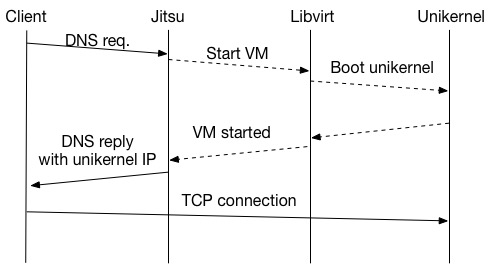
\includegraphics[width=0.8\textwidth]{figures/jitsu.jpg}
    \caption{Jitsu \cite{jitsu}} \label{fig:jitsu}
  \end{figure}
\fi
This project is being used to serve static websites, which is a simple task to do. Nevertheless, their fast boot times allows them to use unikernels instead of docker containers. The DNS server running in that example is also a unikernel, so the environment can be achieved in a pure unikernel fashion.

Another unikernel stack , IncludeOS, writes it's applicatios in C++. C++ is a more industry oriented language than OCaml, but they still have the same network problems. IncludeOS requires an additional file to set up network correctly. It was not easy to set up their hello\_world example flawlessly.

\subsection{Unikernel as Kubernetes Runtime}

Docker is not the only container runtime anymore. The success of Docker led to the creation of Open Container Initiative(OCI). Docker separated their codebase to different modules, called \textit{runC} and \textit{containerd} to create a standart for container runtimes. This standardisation was baked into Kubernetes and now Kubernetes can use different runtimes to run containers. One of those interesting runtimes is \textit{Frakti}, a hypervisor-based container runtime. It uses runV underneath, an OCI runtime to run containers on hypervisors. This is possible by how Kubernetes serves it's runtime specification. A protobuf file \cite{protobuf} the required interface for container runtimes to interact with the Kubernetes master. Similar to virtual-kubelet presented in this research, a new runtime can be created which will be hypervisor-based as the ones discussed above but runs unikernels instead of containers. The interface is very similar to one that is already implemented by virtual-kubelet. For example , the protobuf file has a \textbf{rpc ListContainers(...)} command, which is already implemented for virtual kubelet. 

A complete implementation will run unikernels natively on Kubernetes, removing the need for virtual-kubelet, making unikernel technology truly cloud native. However it requires a more mature and standartised unikernel environment.